\chapter{A model for enhancing the expressiveness of vesting rules}\label{ch:vesting-system}

In this chapter, we will walk through the Alloy model, which enhances upon an open-source JSON Schema model. We incorporate and demonstrate the use of And/Or/Not operators, thus extending the triggers to more of a domain-specific language that supports propositional logic. In particular, we leverage the not operator with the ExactDate trigger to express the ``until condition'', which allows the model to express contract clauses that stipulate a milestone to be achieved until a given date.

The model is shown in Figure~\ref{fig:vs-metamodel}.
\begin{figure}[H]
	\centering
	\fbox{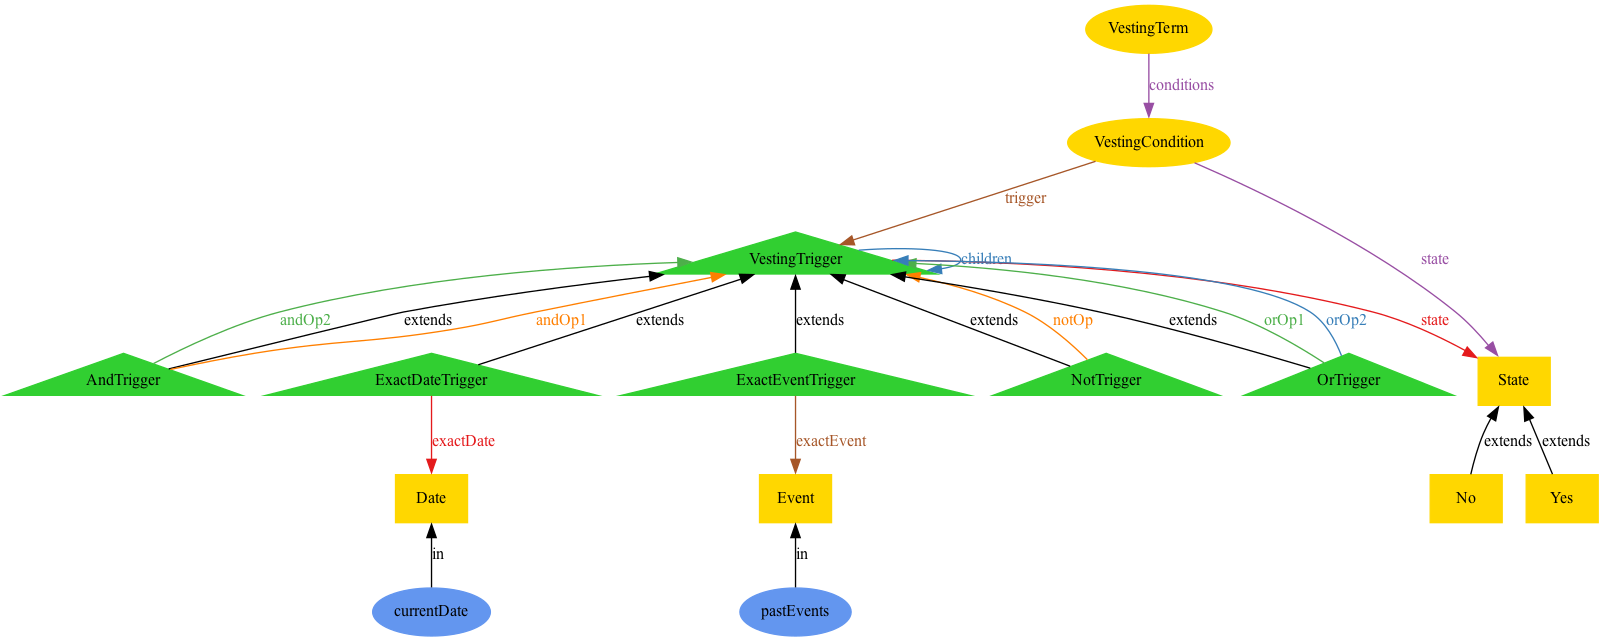
\includegraphics[width=\textwidth]{images/metamodel4.png}}
	\caption{Vesting system metamodel}\label{fig:vs-metamodel}
	As rendered by the Alloy Analyzer
\end{figure}

\section{Vesting Terms and Conditions}

Our Alloy model begins with the definition of the \verb|VestingTerm|, \verb|VestingCondition| and \verb|VestingTrigger| signatures.

A \verb|VestingTerm| represents a set of conditions that need to be met and the authorized shares for the vesting term. The \verb|VestingCondition| signifies a particular condition or a trigger.

Since our modeling has no form of mutation involved, there is no need to identify a vesting term with a vesting condition \textemdash{whether other vesting terms refer to the same conditions is harmless, as long as the authorized shares match the shares in the conditions}.

\begin{listing}[H]\label{listing:vs:vesting-term}
	\begin{minted}{alloy}
	sig VestingTerm {
		conditions : set VestingCondition,
		authorizedShares : Int
	}
	\end{minted}
	\caption{Vesting term signature}
\end{listing}

\begin{listing}[H]\label{fig:vs:vesting-condition}
	\begin{minted}{alloy}
sig VestingCondition {
    trigger : VestingTrigger,
    state : State,
    shares : Int
}
\end{minted}
	\caption{Vesting condition signature}
\end{listing}

This fact relating shares in vesting terms and shares in vesting conditions is not expressible in JSON Schema because it is a constraint that relates two different entities and evaluates arithmetic.

\begin{listing}[H]\label{fig:vs:fact-vesting-condition}
	\begin{minted}{alloy}
fact {
    all t : VestingTerm {
        lte[sum[t.conditions.shares], t.authorizedShares]
    }
}
\end{minted}
	\caption{Fact\textemdash{Only as many shares as authorized can be granted}}
\end{listing}

\section{Vesting Triggers}

\verb|VestingTrigger| is an abstract sig that signifies the state and its children.

\begin{listing}[H]\label{fig:vs:trigger}
	\begin{minted}{alloy}
abstract sig VestingTrigger {
    state : State,
    children : set VestingTrigger
}
\end{minted}
	\caption{The abstract Vesting trigger signature}
\end{listing}

It has four extensions: \verb|ExactDateTrigger|, \verb|ExactEventTrigger|, \verb|AndTrigger|, and \verb|OrTrigger|. \verb|ExactDateTrigger| and \verb|ExactEventTrigger| trigger on an exact date and event, respectively.

\begin{listing}[H]\label{fig:vs:exact-date-trigger}
	\begin{minted}{alloy}
sig ExactDateTrigger extends VestingTrigger {
    exactDate : one Date
} {
    no children
}
\end{minted}
	\caption{Exact date trigger signature}
\end{listing}

\begin{listing}[H]\label{fig:vs:exact-event-trigger}
	\begin{minted}{alloy}
sig ExactEventTrigger extends VestingTrigger {
    exactEvent : one Event
} { 
    no children
}
\end{minted}
	\caption{Exact event trigger signature}
\end{listing}

\verb|AndTrigger| and \verb|OrTrigger| represent the logical AND and OR operations, where the trigger is computed from two other triggers. We further enhance this model by introducing a \verb|NotTrigger|, representing the logical NOT operation.

\begin{listing}[H]\label{fig:vs:and=trigger}
	\begin{minted}{alloy}
sig AndTrigger extends VestingTrigger {
	andOp1 : one VestingTrigger,
	andOp2 : one VestingTrigger - andOp1
} {
	children = andOp1 + andOp2
}
\end{minted}
	\caption{And trigger signature}
\end{listing}

\begin{listing}[H]\label{fig:vs:or-trigger}
	\begin{minted}{alloy}
sig OrTrigger extends VestingTrigger {
    orOp1 : one VestingTrigger,
    orOp2 : one VestingTrigger - orOp1
} {
	children = orOp1 + orOp2
}
\end{minted}
	\caption{Or trigger signature}
\end{listing}

\begin{listing}[H]\label{fig:vs:not-trigger}
	\begin{minted}{alloy}
sig NotTrigger extends VestingTrigger {
    notOp : one VestingTrigger
} {
    children = notOp
}
\end{minted}
	\caption{Not trigger signature}
\end{listing}

\textbf{This is a valuable contribution because it adds a propositional logic layer over the vesting rules in the original model}.


\section{Facts}

Facts establish the truth in our Alloy model. We define facts for \verb|ExactDateTrigger|, \verb|ExactEventTrigger|, \verb|AndTrigger|, \verb|OrTrigger| and \verb|NotTrigger| where we set their state based on the conditions of their triggers~\textemdash{this is how we give the evaluation rules for the vesting triggers}.

\subsection{Evaluation for dates and events}

\begin{listing}[H]\label{list:vs:fact-exact-date-trigger-eval}
	\begin{minted}{alloy}
fact {
	all t : ExactDateTrigger {
		lte[t.exactDate, currentDate] iff t.state = Yes
	}
}
\end{minted}
	\caption{Fact\textemdash{Exact date trigger evaluation}}
\end{listing}

\begin{listing}[H]\label{fig:vs:fact-exact-event-trigger-eval}
	\begin{minted}{alloy}
fact {
	all t : ExactEventTrigger {
		t.exactEvent in pastEvents iff t.state = Yes
	}
}
\end{minted}
	\caption{Fact\textemdash{Exact event trigger evaluation}}
\end{listing}

\subsection{Evaluation for And/Or/Not Triggers}

\begin{listing}[H]\label{fig:vs:fact-and-trigger-eval}
	\begin{minted}{alloy}
fact {
	all t : AndTrigger {
		t.state = Yes iff (t.andOp1.state = Yes and t.andOp2.state = Yes)
	}
}
\end{minted}
	\caption{Fact\textemdash{And trigger evaluation}}
\end{listing}

\begin{listing}[H]\label{fig:vs:fact-or-trigger-eval}
	\begin{minted}{alloy}
fact {
	all t : OrTrigger {
		t.state = Yes iff (t.orOp1.state = Yes or t.orOp2.state = Yes)
	}
}
\end{minted}
	\caption{Fact\textemdash{Or trigger evaluation}}
\end{listing}

\begin{listing}[H]\label{fig:vs:fact-not-trigger-eval}
	\begin{minted}{alloy}
fact {
    all t : NotTrigger {
        t.state = Yes iff t.notOp.state = No
    }
}
\end{minted}
	\caption{Fact\textemdash{Not trigger evaluation}}
\end{listing}

\section{Functions and Checks}

We now introduce several functions to calculate vested and granted shares. The function \verb|vestedShares| returns the number of vested shares, and \verb|grantedShares| returns the number of granted shares for a vesting term. We also introduce checks to ensure that granted shares are greater than or equal to vested shares and that they are positive, and that vested shares are non-negative.

\begin{listing}[H]\label{fig:vs:fun-vested-shares}
	\begin{minted}{alloy}
fun vestedShares[c : VestingCondition] : Int {
    c.state = Yes implies c.shares else 0
}

fun vestedShares[t : VestingTerm] : Int {
    sum c : t.conditions | vestedShares[c]
}
\end{minted}
	\caption{Functions\textemdash{Vested shares}}
\end{listing}

\begin{listing}[H]\label{fig:vs:fun-granted-shares}
	\begin{minted}{alloy}
fun grantedShares[t : VestingTerm] : Int {
    sum c : t.conditions | c.shares
}
\end{minted}
	\caption{Functions\textemdash{Granted shares}}
\end{listing}

\begin{listing}[H]\label{fig:vs:check-granted-shares-gte-vested-shares}
	\begin{minted}{alloy}
check {
    all t : VestingTerm {
        gte[grantedShares[t], vestedShares[t]]
    }  
}

fact {
    all t : VestingTerm {
        lte[sum[t.conditions.shares], t.authorizedShares]
    }
}

check {
    all t : VestingTerm {
        pos[grantedShares[t]]
    }  
}

check {
    all t : VestingTerm {
        nonneg[vestedShares[t]]
    }  
}
\end{minted}
	\caption{Checks\textemdash{Granted shares greater than or equal to vested shares}}
\end{listing}

This modeling approach enables linking to a model very similar to the transaction tracing model by adding \glspl{transaction} similar to \glspl{exercise} that output a new plan \gls{security} with more exercised shares and the same vesting term.

\section{Conclusion}

We improved the semantics of the original model as we translated it to Alloy. Our improvement came out of identifying the space for a propositional logic layer over the original model. We closed the chapter by showing how an instance from our model, when expressed in prose in legal documents, is difficult to understand and analyze.
